% package inclusion does not work, need to figure this out
% \usepackage{url}

% macros for comments
\newcommand{\maren}[1]{{\color{cyan} \textbf{[Maren: #1]}}}
\newcommand{\andrei}[1]{{\color{red} \textbf{[Andrei: #1]}}}
\newcommand{\rev}[1]{{\color{blue} \textbf{#1}}}

\section{Introduction \label{introduction}}


\maren{Regarding the title of the paper: The UQ comes from the model backend and not from Emukit. Emukit takes a model that is capable of some kind of UQ and uses this capability for active data selection. So Emukit `actifies' the model, yielding an active learning method. The title may suggest that Emukit provide models with UQ capability which is does not. Thoughts on this?}
\andrei{Makes sense! I don't think we have any leeway with the title though, because this is an approved title of the conference talk.}

A few general words about ML, statistical emulation, UQ, and software for those.

\andrei{Testing out macroses}

\maren{Let's also briefly introduce and summarize the unique features of Emukit here. These are
  \begin{itemize}
  \item Model agnosticism 
  \item Using same model for different purposes
  \item Flexibility (quick prototyping)
  \item ...
  \end{itemize}
These should/could then be elaborated on later, perhaps in dedicated subsection with example code.
}

\section{Background on UQ methods}
Here we should give a quick intro into BayesOpt, BQ, design of experiments. Also maybe GPs and multi-fidelity modelling.

\section{Emukit workflow}
Decision making with statistical emulation consists of three parts. All starts with a \textit{task}, a high level goal that we are interested in achieving. It usually involves a complex process that we aim to study and answer a question about. Some examples include finding the best operation mode of a drone, measuring the quality of a weather simulation, explaining behavior of a complex system. In order to solve the task we choose a \textit{method}, a relatively low-level technique that guides our exploration of the targte process and provides the quantifiable way to answer the task's question. Examples include Bayesian optimization, Bayesian quadrature and experimental design. And finally there is a \textit{model}, a probabilistic data-driven representation of the process under study. Consequently, the typical workflow for users working with Emukit consists of three steps (see Figure~\ref{figure:workflow} for a graphical description).

\textbf{Build the model.} Instead of constraining the user to certain model classes, Emukit provides the flexibility of using user-specified models. Generally speaking, Emukit does not provide modelling capabilities. Instead users are expected to define their own models. Because of the variety of modelling frameworks available, Emukit does not mandate or make any assumptions about a particular modelling technique or a library, and suggests to implement a subset of defined model interfaces that are required to use a particular method.

\textbf{Run the method.} This is the main focus of Emukit. Emukit defines a general structure of a decision making method and offers implementations of several such methods: Bayesian optimization, Bayesian quadrature, experimental design, and sensitivity analysis. All methods are model-agnostic and only rely model interfaces.

\textbf{Solve the task.} For the end users, Emukit is a way to solve a certain task, which may have research or business value. Emukit provides a set of examples of how tasks such as hyper-parameter tuning, sensitivity analysis multi-fidelity modelling or benchmarking are accomplished using the library.

\begin{figure}[h]
    \centering
      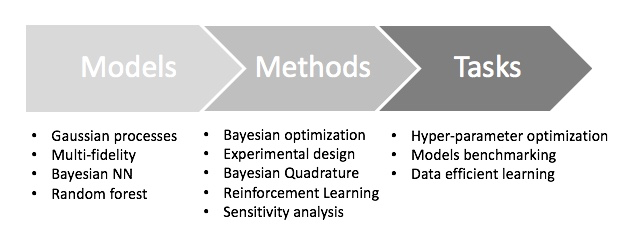
\includegraphics[scale=0.4]{workflow.png}  
    \caption{Summary of workflow for the users of Emukit. A model is computed in modelling framework of choice. The model is wrapped using a pre-defined interface and connected to the core components of several methods such as Bayesian optimization, experimental design etc. Specific tasks are then solved using these methods.}
    \label{figure:workflow}
\end{figure}

\section{Architecture of the Emukit package}
\maren{Can we rename the section title to package design or sth like this? To a ML researcher `design' would be the node design. (I know these are not ML proceedings but it's still confusing)}
\andrei{Sure thing, renamed, although this is probably not ideal either.}

At a conceptual level the methods supported in Emukit -- such as Bayesian optimisation, experimental design and quadrature -- are all cyclic decision making processes that follow a similar pattern.\maren{It may be good to simply use the defined names `Bayesian optimization' and `Bayesian quadrature' as not all optimization or quadrature methods are Bayesian. Also, it is not true that e.g., all Bayesian quadrature methods and all exp design methods are cyclic (it is true for BO though). The term Bayesian learning methods seems a bit ill-suited. We could perhaps talk about active learning/active point selection for probabilistic models (some of which are Bayesian).} \andrei{Fair enough, I just invented something on the go. But it would be very convenient to have a collective name.}
Algorithmically they can be thought of as instances of a common abstract loop, which we now describe (also described by Algorithm \ref{alg:emukit_loop}).

The common goal of all these methods is to learn a behavior of an \textit{objective function} - a black box expensive process that has certain \textit{parameters}. The knowledge about the objective function (initially available as well as that collected during the learning process) is represented with a \textit{probabilistic model}. A mechanism employed to propose new data points to evaluate the objective at is called an \textit{acquisition function}. Finally, the decision making process is done in a \textit{loop} until a certain \textit{stopping condition} is met. 

\andrei{Still struggling to understand how to add commands to the preamble, could be that the template doesn't allow that at all. That's limiting, e.g. we cannot use packages for algorithms.}\maren{That's annoying. If there is no solution we can compile the code in another tex file and include a figure of the pseudo-code.}
% Algorithm is taken from the original NeurIPS workshop paper
% \begin{algorithm}
    % \While{stopping condition is not met}{
    %     collect next point(s) for evaluation\;
    %     evaluate objective function\;
    %     update model with new observation(s)\;
    % }
    % \caption{Decision making loop in Emukit}
    % \label{alg:emukit_loop}
% \end{algorithm}

The internal structure of Emukit reflects these abstractions to ensure that fundamental components of the decision making loop could be swapped out and replaced. While some of the basic components in Emukit correspond to the parts of the Bayesian decision making loop exactly, others are more fine-grained to allow for greater flexibility and plug-and-play experience for the researchers using the package. We will now give an overview of these components.

\andrei{Below is largely based on our documentation}
\textbf{Outer Loop}. The \texttt{emukit.core.loop.OuterLoop} class is the abstract loop where the different components come together. Loops for specific methods, such as Bayesian optimisation and experiment design, should subclass it.

\textbf{Parameter space}. Represents parameter space of the objective function. Emukit supports continuous, categorical, discrete, and bandit parameters.

\textbf{Model}. All Emukit loops need a probabilistic model. Emukit does not provide functionality to build models as there are already good modelling frameworks available in Python. Instead, it provides a way of interfacing third part modelling libraries. The interfacing mechanism consists of two parts: interfaces and wrappers. \textit{Interfaces} define functionality required from a model Different models and modelling frameworks will provide different functionality. For instance a Gaussian process will usually have derivatives of the predictions available but random forests will not. These different functionalities are represented by a set of interfaces which a model implements. The basic interface that all models must implement is \texttt{IModel}, which implements functionality to make predictions and update the model but a model may implement any number of other interfaces such as \texttt{IDifferentiable} which indicates a model has prediction derivatives available. Interfaces can also be defined by other components of the decision making loop to indicate that a certain functionality is required from the model. For example, \texttt{ICalculateVarianceReduction} defines methods the user needs to implement with their model to use it with the vadirance reduction technique. \texttt{Model wrappers} adopt third-party models and implement one or more of the interfaces using specific modelling framework. Emukit provides a wrapper for using a model created with \texttt{GPy} \cite{gpy2014}.

\maren{I find the interface capability of Emukit quite unique and a real selling point. It somehow gets lost a bit in between the lines. Shall we make a separate section called `model interfaces' or `custom backends' or sth similar with an example and simply mention here briefly that models are big interfaced?}

\textbf{Candidate Point Calculator}. This entity drives the decision on which point(s) to evaluate next. The simplest implementation provided out of the box, \texttt{SequentialPointCalculator}, collects one point at a time by finding where the acquisition is at a maximum by applying the acquisition optimiser to the acquisition function. More complex implementations are possible, for example to enable batches of points to be collected so that the user function can be evaluated in parallel.

\textbf{Acquisition}. The acquisition is a function defined on the parameter space that produces continuous values. It represents a heuristic quantification of how valuable collecting a future point might be, and produces continuous values.It is used by the candidate point calculator to decide which point(s) to collect next. Acquisition functions balance exploration and explotation of the decision making process.

\textbf{Acquisition Optimizer}. The \texttt{AcquisitionOptimizer} optimizes the acquisition function to find the point at which the acquisition is at a maximum. If available, the optimizer can use the acquisition function gradients. Otherwise, it will either estimate the gradients numerically, or use a gradient free optimisation.

\textbf{User Function}. This is the component that represents the objective function. It can be evaluated by the user, or it can be passed into the loop and evaluated by Emukit.

\textbf{Model Updater}. The \texttt{ModelUpdater} class updates the model with new training data after a new point is observed and optimizes any hyper-parameters of the model. It can decide whether hyper-parameters need updating based on some internal logic.

\textbf{Stopping Condition}. The \texttt{StoppingCondition} class chooses when the decision making loop should stop collecting points. The most commonly used example is to stop when a set number of iterations have been reached.

These are the core components Emukit defines. Specific methods can also define additional concepts of their own, e.g. integration measures or cost. Table \ref{table:abstraction_mapping} shows the mapping between Bayesian decision making abstractions and Emukit components.

\begin{table}
    \setlength{\DUtablewidth}{\tablewidth}
    \begin{longtable}[c]{p{0.4\DUtablewidth}p{0.4\DUtablewidth}}
        \toprule
        \textbf{Bayesian decision making abstractions} & \textbf{Emukit components} \\
        \midrule
        \endfirsthead
        Loop & Outer loop \\
        \midrule
        Parameters & Parameter space \\
        Probabilistic model & Model interface \\
        & Model wrapper \\
        \midrule
        Acquisition function & Candidate Point Calculator \\
        & Acquisition \\
        & Acquisition optimiser \\
        \midrule
        Objective function & User function \\
        & Model Updater \\
        \midrule
        Stopping Condition & Stopping condition \\
        \bottomrule
    \end{longtable}
    \caption{The mapping between abstractions of the Bayesian decision making process and the components defined in Emukit.}
    \label{table:abstraction_mapping}
\end{table}

\section{Methods}
In this section we show case Emukit's high level APIs for all main funcitons of the package: Bayesian optimisation, Bayesian quadrature, experimental design, mutli-fidelity emulation. Unless stated otherwise, we assume some initial data (e.g. three-four data points) is already defined and stored in variables \texttt{X} (inputs) and \texttt{Y} (outputs). We use GPy \cite{gpy2014} in the code snippets below for modelling, and exclude lines that import Emukit classes for brevity.

Interfaces for Bayesian optimisation and experimental design are the most straighforward way to use the library. Both methods require the user to define a model and wrap it in the Emukit's model wrapper. Input space also has to be defined using Emukit's classes. The choice of acquisition function is optional, as reasonable defaults are provided. High level loop objects allow the user to execute the decision making loop and access its properties.

\begin{verbatim}
  parameter_space = ParameterSpace([
      ContinuousParameter('x1', -5, 10),
      ContinuousParameter('x2', 0, 15)
  ])
  model_gpy = GPy.models.GPRegression(X,Y)
  model_emukit = GPyModelWrapper(model_gpy)

  expected_improvement_acquisition =
      ExpectedImprovement(model = model_emukit)
  bayesopt_loop = BayesianOptimizationLoop(
      model = model_emukit,
      space = parameter_space,
      acquisition = expected_improvement_acquisition
  )

  model_variance_acquisition =
      ModelVariance(model = model_emukit)
  experimental_design_loop =
      ExperimentalDesignLoop(
          model = model_emukit,
          space = parameter_space,
          acquisition = model_variance
      )
\end{verbatim}

Usage of Bayesian quadrature (BQ) API is more envolved, as even in its most basic form it requires more design choices from the user. First the objective function, also referred to as an integrand, is modelled with a Gaussian process (GP). Since BQ integrates the kernel function, the kernel is then wrapped in a separate Emukit object. Bundled together, wrappers around the kernel and the model itself represent a base model in the BQ package. This model can be used with several BQ methods, the code below illustrates vanilla Bayesian quadrature where the GP model is directly placed over the integrand function and then integrated analytically.

\begin{verbatim}
  lb = -3. # lower integral bound
  ub = 3. # upper integral bound
  gpy_model = GPy.models.GPRegression(X=X, Y=Y)

  emukit_rbf = RBFGPy(gpy_model.kern)
  emukit_qrbf = QuadratureRBF(
      emukit_rbf,
      integral_bounds=[(lb, ub)]
  )
  emukit_model = BaseGaussianProcessGPy(
      kern=emukit_qrbf,
      gpy_model=gpy_model
  )

  emukit_method = VanillaBayesianQuadrature(
      base_gp=emukit_model
  )
  emukit_loop = VanillaBayesianQuadratureLoop(
      model=emukit_method
  )
\end{verbatim}

Once the loop object is created, either for optimisation, quadrature or experiment design, it can be evaluated in one of two modes. If the user has access to the objective function via Python, the loop can be managed by Emukit with the \texttt{run\_loop} method that accepts two arguments: the objective function and the stopping criterion. If the objective has to be called externally (e.g. a lab experiment has to be done), Emukit provides \texttt{get\_next\_points} method that produces the next evaluation point(s) based on the data observed so far. In that latter case user has to manage the decision making loop themselves.

To support research on multi-fidelity emulation methods, Emukit implements both linear and non-linear multi-fidelity models. The user is expected to bring data for each of the fidelities and make the choice of appropriate Gaussian process kernel. Emukit can then be used to define a combined multi-fidelity model. In the example below a define a linear model.

\begin{verbatim}
  # This utility method allows to
  # convert data from different fidelities
  # to arrays where fidelity is represented
  # as an input variable
  X, Y = convert_xy_lists_to_arrays(
      [x_low, x_high],
      [y_low, y_high]
  )

  kernels = [
      GPy.kern.RBF(dim=1),
      GPy.kern.RBF(dim=1)
  ]
  linear_mf_kernel =
      LinearMultiFidelityKernel(kernels)
  gpy_linear_mf_model =
      GPyLinearMultiFidelityModel(
          X, Y,
          linear_mf_kernel,
          n_fidelities = 2
  )
\end{verbatim}

In addition to the APIs discussed above, Emukit also provides basic support for sensitivity analysis and benchmarking. Further information about Emukit's functionality, including available implementations of acquisition functions, multi-output models, support for constraints and cost functions, custom events in the outer loop, etc., can be found on library's website\footnote{\url{https://emukit.github.io/}}, documentation\footnote{\url{https://emukit.readthedocs.io/en/latest/}} and tutorial notebooks\footnote{\url{https://nbviewer.org/github/emukit/emukit/blob/main/notebooks/index.ipynb}}. 

\maren{May it be useful to introduce each of the methods (BO, BQ, ExpDesign) with some minimal example code similarly to the webpage? }
\andrei{Good idea! Did the first pass.}

\section{Examples of usage}
Since its announcement in 2019 \cite{paleyes2019emulation}, Emukit was used in a wide range of research projects. In this section we review a selection of these projects to showcase the breadth of situations in which the library can be useful.

\subsection{Methodological research}
Because of its flexibility Emukit allows researchers to rapidly experiment with decision making methods in Emukit's suite. In this section we discuss several papers that leverage this fact.

Optimisation of parameters in high dimensional structured data spaces is an increasingly important and challenging task. A common pattern is to use unsupervised learning methods to project parameters into low dimensional continuous representations, also known as latent spaces. There are multiple ways to approach the design the Bayesian optimisation procedure on such latent spaces. Siivola et al. \cite{siivola2021good} study the effects of various design choices. Namely, the effects of the dimensionality of the latent space, the optimisation bounds, and the choice of acquisition function are analyzed. Emukit's plug-and-play design allowed the researchers to facilitate an efficient comparison of these components in isolation, without affecting the rest of the the optimisation loop.

\andrei{Maren, would you like to write a paragraph about your work on BQ with Alex G.? Or the one with Masha? Or both?}

\subsection{Applications}
In this section we describe several cases where Emukit was used to solve a problem in other scientific domains.

Bell et al. used Emukit to show how to conduct multiverse analysis for machine learning experiments \cite{bell2022modeling}. Multiverse analysis was originally introduced in psychology, and allows researchers to explore the robustness and generality of claims by systematically examining the impact of different choices and variations in the experimental setup. The authors argue that the same concept can be applied to the machine learning: if a new technique, e.g. batch normalization, is proposed for an ML model, it should remain effective regardless of the model architecture, optimization method, dataset, evaluation metric, and so on. The set of these variations comprises a multiverse, and needs to be explored effectively. The authors surrogate modelling and Bayesian experimental design to efficiently systematically explore the effect of each choice. Emukit was chosen as an implementation tool because of the experimental design API it provides.

Uhrenholt and Jensen used Emukit's Bayesian optimisation module to solve the problem of finding settings of a musical synthesizer to produce a given sound \cite{uhrenholt2019efficient}. A musical synthesizer produces sound by generating waveforms via oscillators. Created audio streams are then routed through a pipeline that consists (not necessary all) of mixing of separate streams, filtering, adding of noise, and saturation. Musicians can control the output sound by changing the configuration of the pipeline. In order to estimate the discrepancy between the produced sound and the target, the authors designed a novel modeling approach, in which Gaussian process is used to model the distribution of the output's L2 norm. The flexibility of Emukit allowed to implement this customization directly, without necessary effort duplication. Emukit's API also facilitated a fair comparison to standard Bayesian optimization baseline.

Liyanage et al. faced the problem of combining data from multiple particle accelerators, including Large Hadron Collider and Relativistic Heavy Ion Collider, to study the properties of quark-gluon plasma \cite{PhysRevC105034910}. Nuclear collision experiments generate a large body of measurements with varying levels of uncertainty that would be expensive to quantify with simulations. Instead the authors proposed to use inexpensive statistical emulators and use transfer learning to leverage similarities between different heavy ion collisions systems. This new technique is based on multi-fidelity emulation, making Emukit an obvious implementation choice.

\section{Related work}
Python ecosystem is rich with powerful scientific packages, including those that cover decision making methods. In particular, Bayesian optimisation enjoys a wide selection of tools and frameworks. Spearmint \cite{snoek2012practical} and GPyOpt \cite{gpyopt2016} are among the first Python packages for Bayesian optimisation, the latter being an inspiration for the first release of Emukit. BoTorch \cite{balandat2020botorch} is a popular library for Bayesian optimisation based on PyTorch. Similarly, Trieste \cite{picheny2023trieste} also focuses on Bayesian optimisation but uses Tensorflow as a backend. More options, such as pyGPGO \cite{jimenez2017pygpgo}, scikit-optimize \cite{louppe2017bayesian}, RoBO \cite{klein-bayesopt17} are also available. For other methods supported by Emukit the choice of frameworks is more scarce. Namely, bayesquad \cite{Charles2013} appears to be the only other usable Python package for Bayesian quadrature. Optbayesexpt \cite{mcmichael2021optbayesexpt} and NEXTorch \cite{wang2021nextorch} provide Bayesian experimental design functional adopted for their respective fields. Elements of Bayesian experimental design can also be found in Trieste \cite{picheny2023trieste}. The key difference between Emukit and mentioned libraries is the fact that Emukit does not dictate a particular modelling framework, allowing for flexibility in choice of computational backends.

Likewise, to the best of our knowledge Emukit remains the only Python library to provide multi-fidelity emulation functionality. Another notable package for research on multi-fidelity methods is MF2 \cite{vanRijn2020} that implements a variety of multi-fidelity benchmark functions.

Looking at a wider family of optimisation libraries in Python, Optuna \cite{optuna_2019} is a popular choice for hyperparameter optimisation. Similarly to Emukit, Optuna is framework agnostic, however it provides a different set of optimisation methods, focusing on evolutionary, genetic and Monte Carlo based approaches. Finally, Ray Tune \cite{liaw2018tune} is a well known scalable platform in Python on which other model optimisation frameworks can be executed. Emukit can potentially be integrated with Ray Tune as an optimisation library. This work was not carried out yet, and can be a future development direction.


\andrei{Maren, shall we mention Probnum here somehow?}
\andrei{I've think this section should focus on Python libs only. So no clients for cloud services (e.g. Vizier or SageMaker) and no libraries in R, Julia and such. Sounds good?}

\section{Conclusion}
we conclude the paper. maybe future work goes here? we don't have anything big planned

\section{Acknowledgments}
MM gratefully acknowledges financial support by the European Research Council through ERC StG Action 757275 / PANAMA; the DFG Cluster of Excellence “Machine Learning - New Perspectives for Science”, EXC 2064/1, project number 390727645; the German Federal Ministry of Education and Research (BMBF) through the T\"{u}bingen AI Center (FKZ: 01IS18039A); and funds from the Ministry of Science, Research and Arts of the State of Baden-W\"{u}rttemberg.
